% ============================================================
% 第二章 LaTeX基础示例
% ============================================================

\chapter{LaTeX基础示例}

\section{图片插入示例}

图~\ref{fig:neural-network}展示了一个深度神经网络结构示例。图~\ref{fig:subfig-example}展示了子图排版功能。

% 单图示例（非浮动，严格跟随正文）
\begin{herefig}
    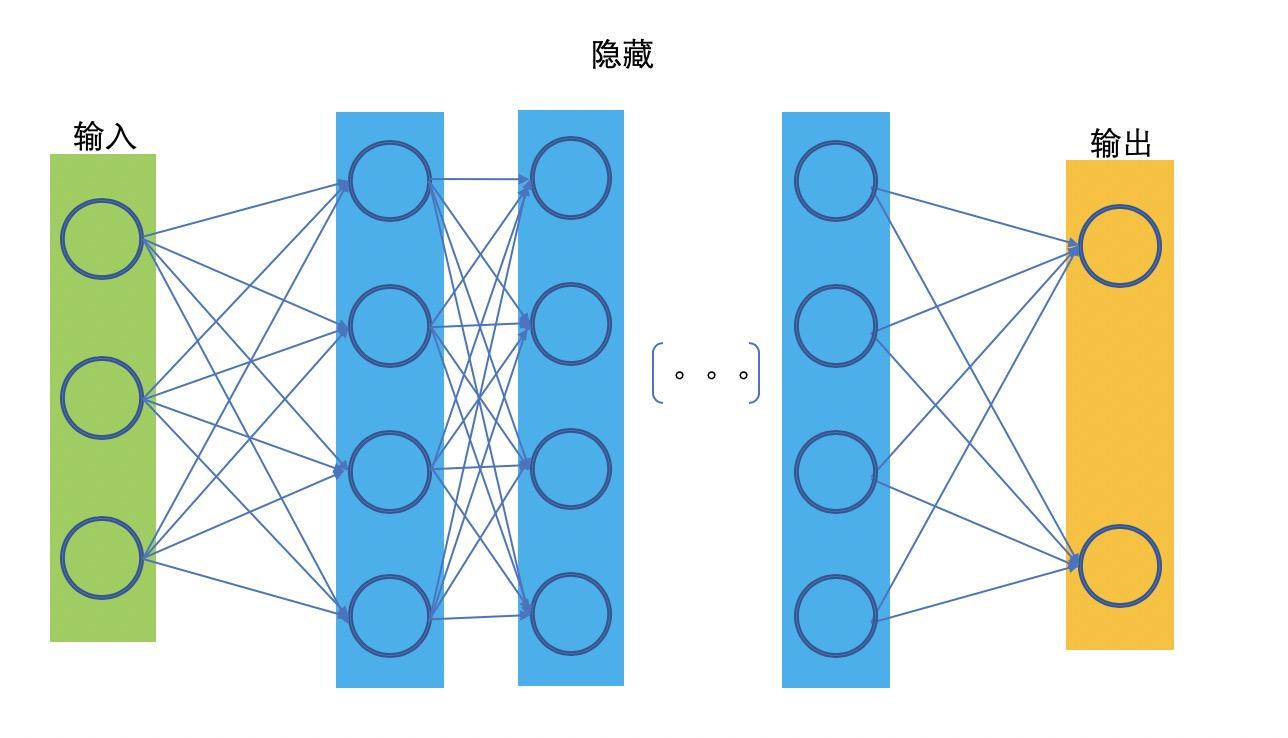
\includegraphics[width=0.8\textwidth]{figture/example}
    \bicaption{深度神经网络结构示意图}{Schematic Diagram of Deep Neural Network Structure}
    \label{fig:neural-network}
\end{herefig}

% 子图示例（非浮动，严格跟随正文）
\begin{herefig}
    \begin{subfigure}[t]{0.48\textwidth}
        \centering
        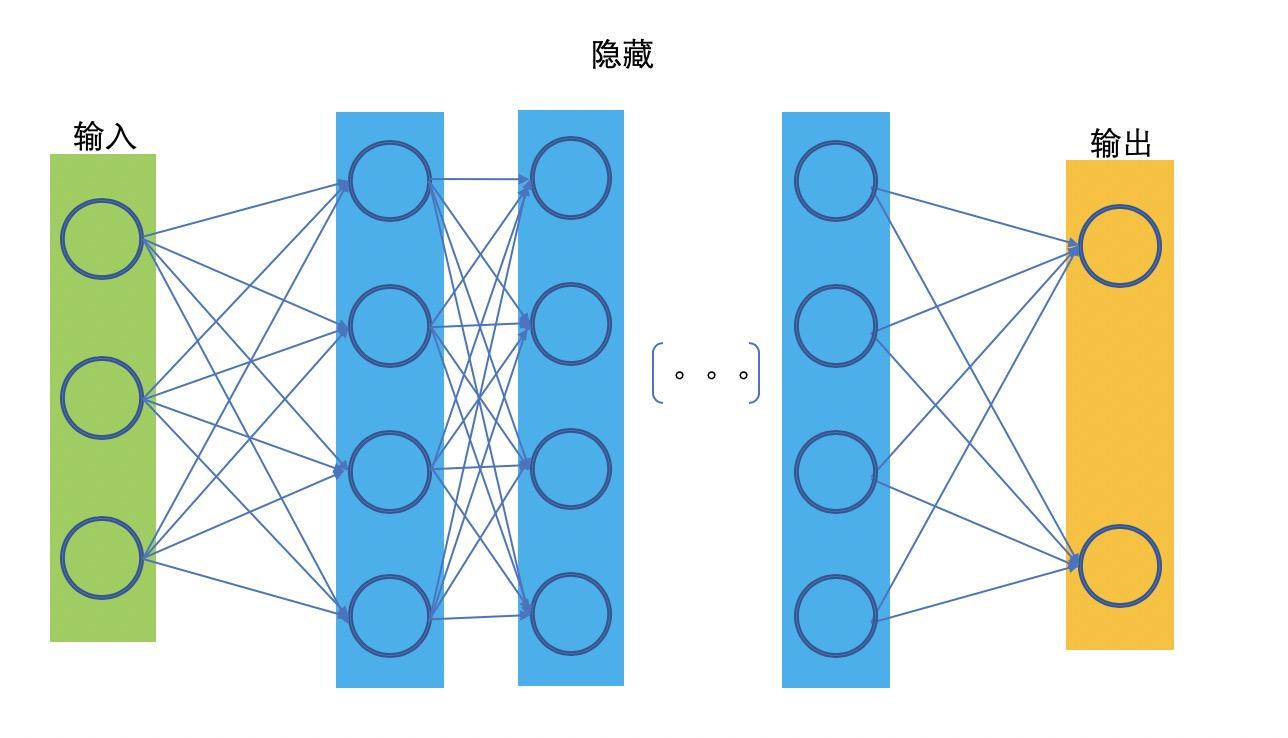
\includegraphics[width=0.9\linewidth]{figture/example}
        \bicaption{子图A说明}{Subfigure A Description}
        \label{fig:sub-a}
    \end{subfigure}
    \hfill
    \begin{subfigure}[t]{0.48\textwidth}
        \centering
        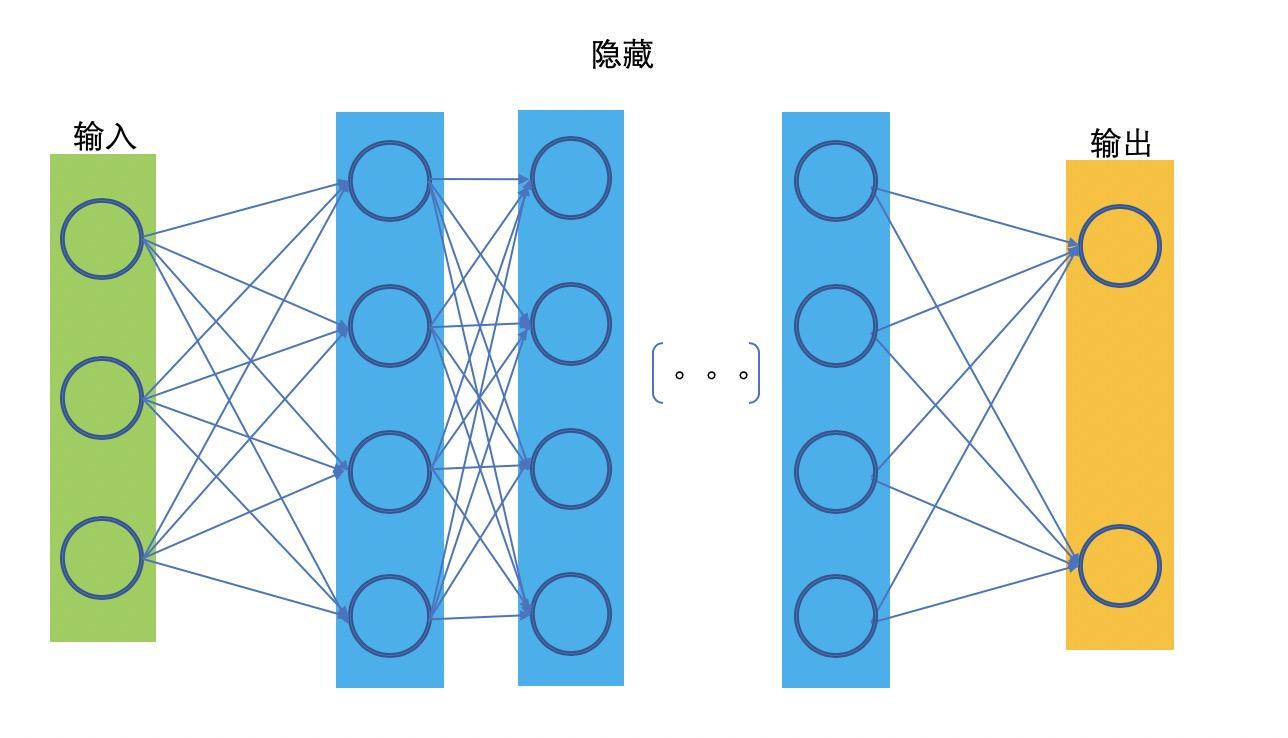
\includegraphics[width=0.9\linewidth]{figture/example}
        \bicaption{子图B说明}{Subfigure B Description}
        \label{fig:sub-b}
    \end{subfigure}
    \bicaption{子图排版示例}{Example of Subfigure Layout}
    \label{fig:subfig-example}
\end{herefig}

\section{公式排版示例}

行内公式示例：$E = mc^2$，$\alpha + \beta = \gamma$。

独立编号公式示例：
\begin{equation}
    \int_{a}^{b} f(x) \, dx = F(b) - F(a)
    \label{eq:integral}
\end{equation}

多行对齐公式示例：
\begin{align}
    \nabla \cdot \vec{E} &= \frac{\rho}{\varepsilon_0} \label{eq:maxwell1} \\
    \nabla \times \vec{E} &= -\frac{\partial \vec{B}}{\partial t} \label{eq:maxwell2}
\end{align}

公式~\eqref{eq:integral}展示了微积分基本定理，公式~\eqref{eq:maxwell1}和\eqref{eq:maxwell2}是麦克斯韦方程组的一部分。

\section{表格排版示例}

表~\ref{tab:three-line}展示了标准三线表的排版效果。

% 三线表示例（非浮动短表格，严格跟随正文）
\begin{heretab}
    \bicaption{实验结果对比表}{Comparison of Experimental Results}
    \label{tab:three-line}
    \begin{tabular}{ccc}
        \toprule
        \textbf{方法} & \textbf{准确率(\%)} & \textbf{运行时间(s)} \\
        \midrule
        方法A & 92.5 & 1.23 \\
        方法B & 94.8 & 1.56 \\
        方法C & 96.2 & 2.01 \\
        \bottomrule
    \end{tabular}
\end{heretab}

表~\ref{tab:multi-row}展示了包含多行合并的表格。

\begin{heretab}
    \bicaption{多层结构数据表}{Multi-level Structure Data Table}
    \label{tab:multi-row}
    \begin{tabular}{cccc}
        \toprule
        \textbf{类别} & \textbf{参数} & \textbf{数值} & \textbf{单位} \\
        \midrule
        \multirow{2}{*}{输入} & 通道数 & 3 & - \\
                              & 尺寸 & 224$\times$224 & px \\
        \midrule
        \multirow{2}{*}{输出} & 类别数 & 1000 & - \\
                              & 概率 & 0.85 & - \\
        \bottomrule
    \end{tabular}
\end{heretab}

\section{跨页长表格示例}

表~\ref{tab:long}展示了可跨页的长表格。当表格超过一页时，下页会自动重复表头，并在右上方标注"续表"，符合三线表规范。

\begin{longtable}{ccc}
    \caption{跨页长表格示例} \label{tab:long} \\
    \toprule
    \textbf{序号} & \textbf{参数名称} & \textbf{数值} \\
    \midrule
    \endfirsthead
    
    \continuedcaption{3}
    \toprule
    \textbf{序号} & \textbf{参数名称} & \textbf{数值} \\
    \midrule
    \endhead
    
    \bottomrule
    \endfoot
    
    \bottomrule
    \endlastfoot
    
    1 & 学习率 & 0.001 \\
    2 & 批大小 & 32 \\
    3 & 迭代次数 & 100 \\
    4 & 隐藏层数 & 3 \\
    5 & 激活函数 & ReLU \\
    6 & 优化器 & Adam \\
    7 & 损失函数 & 交叉熵 \\
    8 &  dropout率 & 0.5 \\
    9 & 正则化系数 & 0.0001 \\
    10 & 输入维度 & 784 \\
    11 & 输出维度 & 10 \\
    12 & 卷积核大小 & 3$\times$3 \\
    13 & 池化尺寸 & 2$\times$2 \\
    14 & 步长 & 1 \\
    15 & 填充 & Same \\
    16 & 学习率衰减 & 0.95 \\
    17 & 早停耐心值 & 10 \\
    18 & 验证集比例 & 0.2 \\
    19 & 测试集比例 & 0.1 \\
    20 & 随机种子 & 42 \\
    21 & 权重初始化 & He \\
    22 & 偏置初始化 & 零初始化 \\
    23 & 批量归一化动量 & 0.1 \\
    24 & 批量归一化 epsilon & 1e-5 \\
    25 & 学习率预热步数 & 500 \\
    26 & 梯度裁剪阈值 & 1.0 \\
    27 & 标签平滑系数 & 0.1 \\
    28 & 数据增强概率 & 0.5 \\
    29 & 旋转角度范围 & $\pm15°$ \\
    30 & 水平翻转概率 & 0.5 \\
    31 & 垂直翻转概率 & 0.0 \\
    32 & 颜色抖动因子 & 0.2 \\
    33 & 高斯噪声标准差 & 0.01 \\
    34 & 随机擦除概率 & 0.25 \\
    35 & Mixup 系数 & 0.2 \\
    36 & CutMix 系数 & 1.0 \\
    37 & 模型参数量 & 25.6M \\
    38 & FLOPs & 4.1G \\
    39 & 训练显存占用 & 8.2GB \\
    40 & 推理显存占用 & 2.1GB \\
    41 & 训练时间/epoch & 45s \\
    42 & 推理时间/样本 & 3.2ms \\
    43 & 模型大小 & 98.5MB \\
    44 & 量化精度 & INT8 \\
    45 & 部署框架 & ONNX \\
\end{longtable}

\section{本章小结}

本章展示了LaTeX模板的核心功能：图片插入（含子图）、数学公式排版（行内公式、独立公式、多行对齐公式）、三线表排版，以及中英双语图表标题功能。
